\lecture{3}{11. Februar 2025}{Stoffer og Tilstandsstørrelser}

\section{Fasesr for kemisk homogene stoffer}

\begin{figure} [ht]
  \centering
  \caption{p-V diagram for vand}
  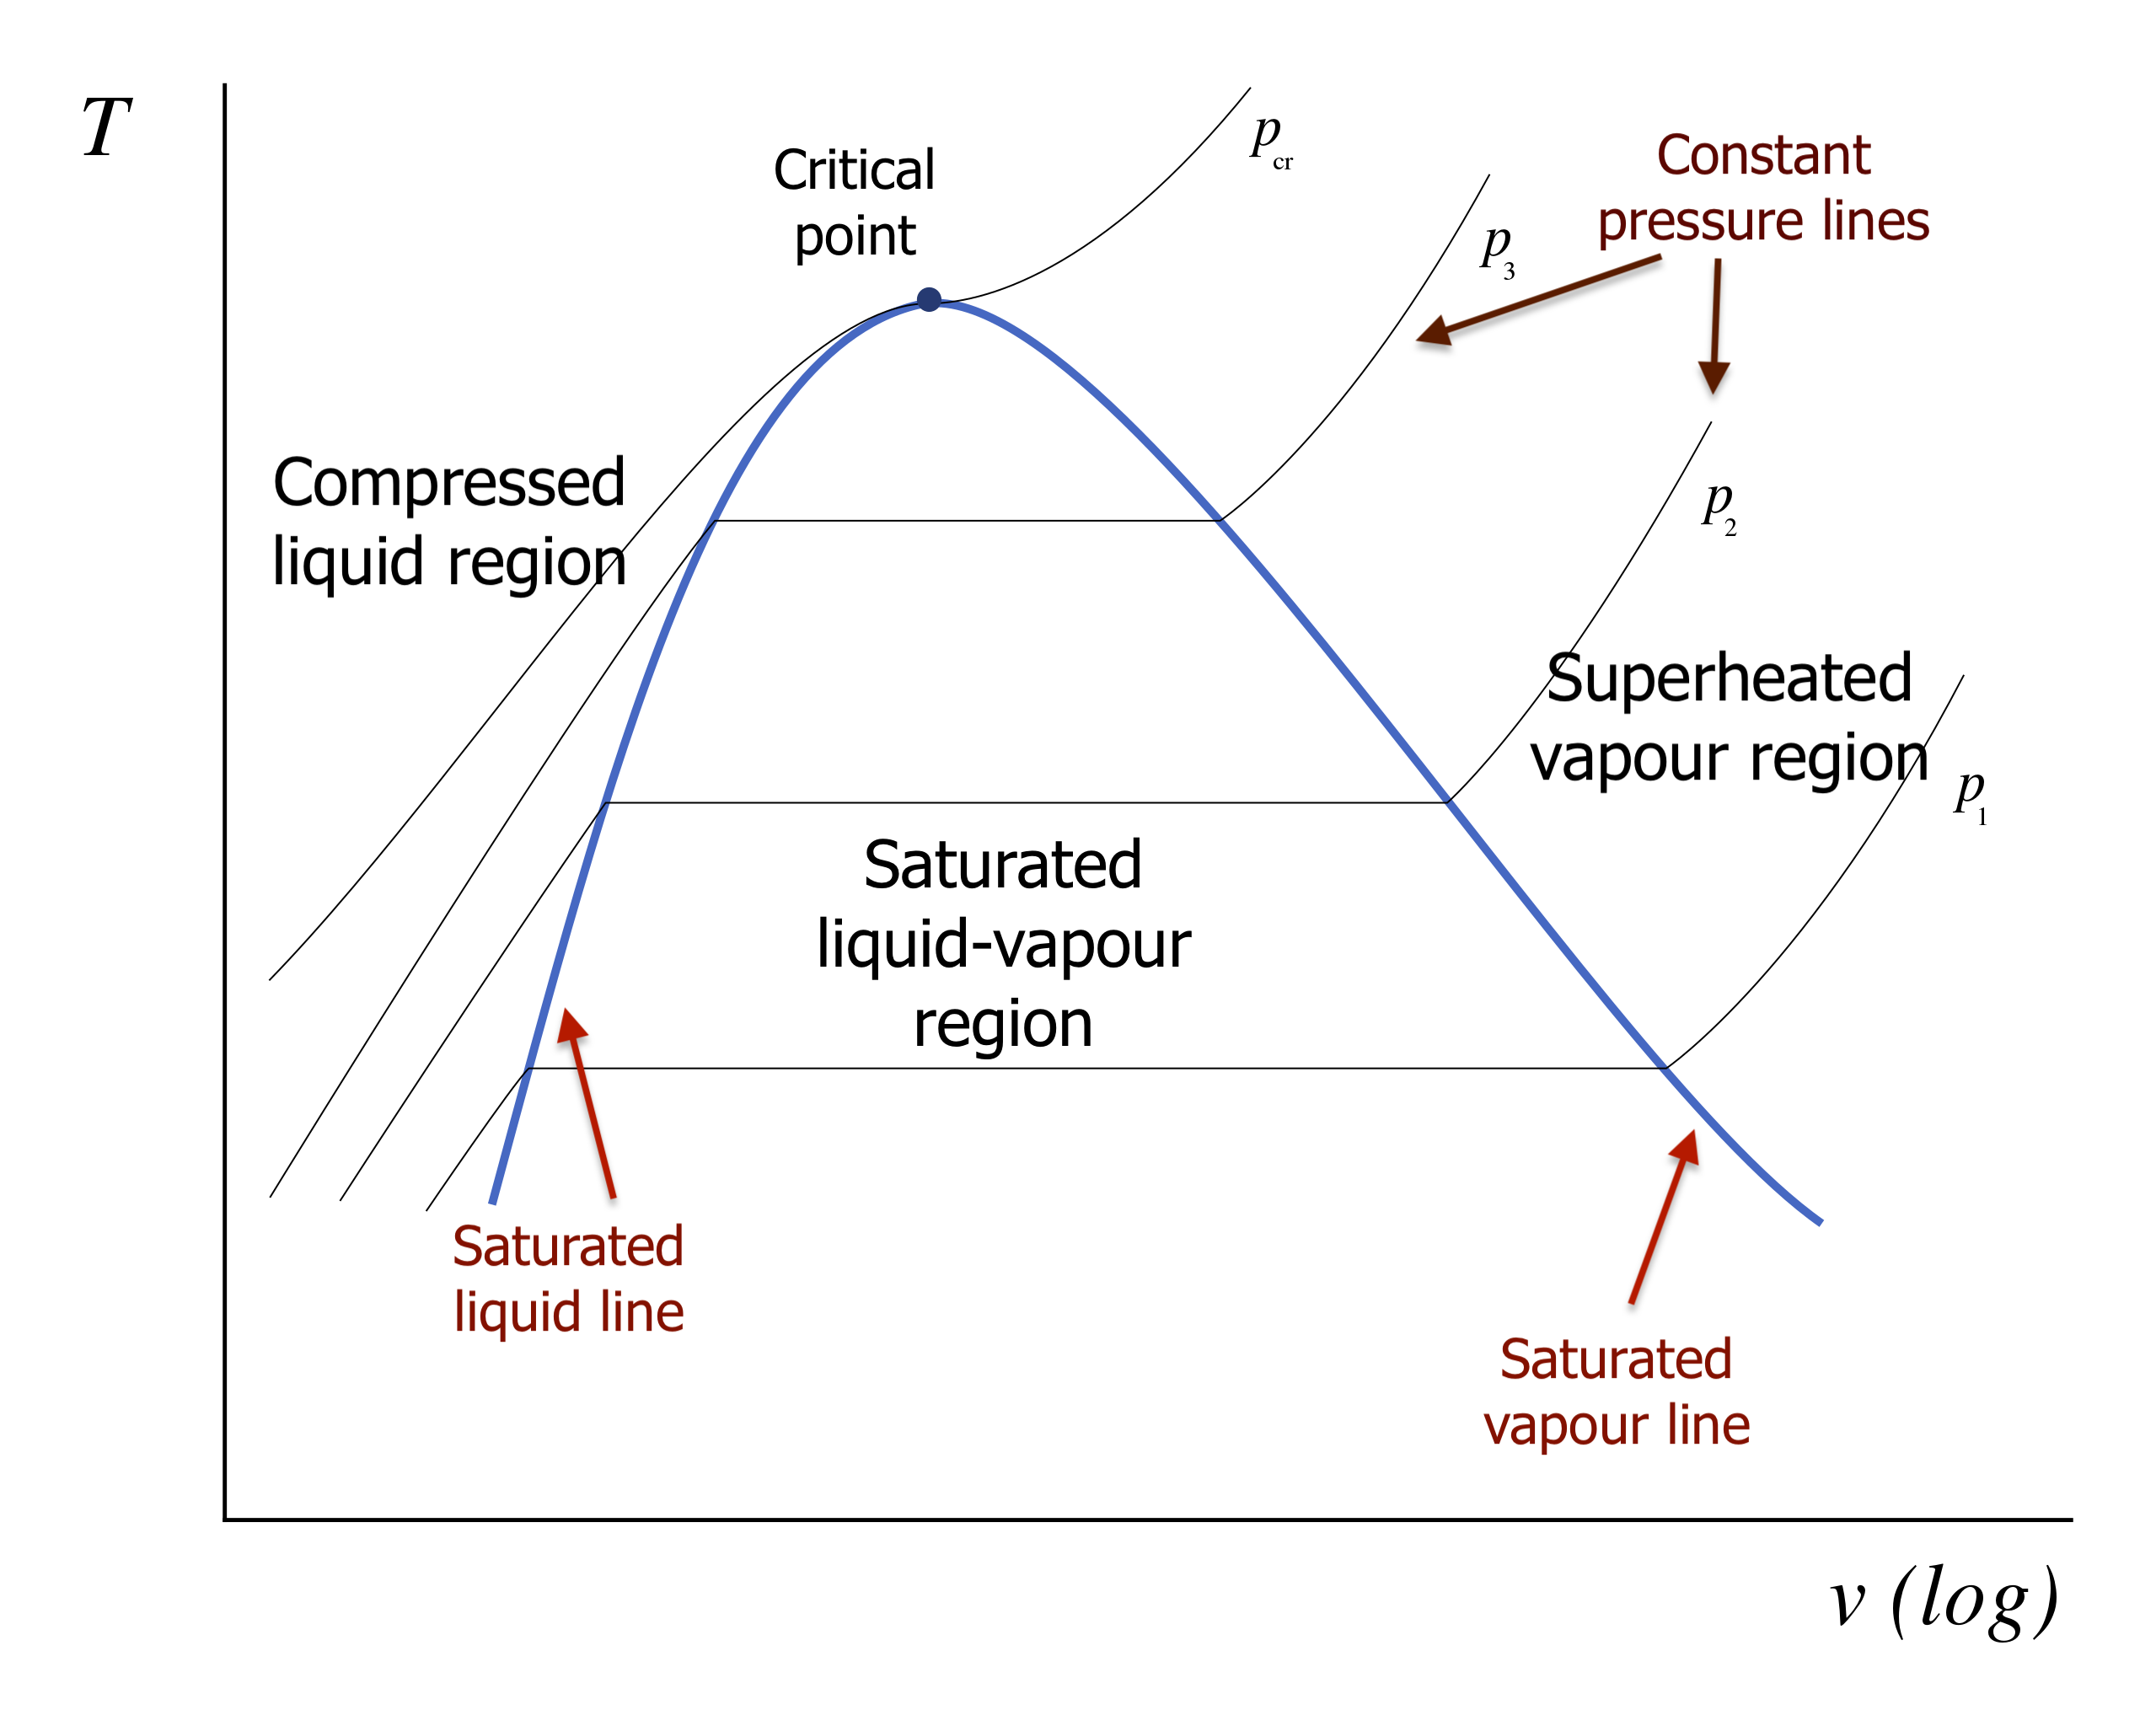
\includegraphics[width=0.5\linewidth]{./figures/f3_1.png}
  \label{fig:f3_1}
\end{figure}
På \textbf{\autoref{fig:f3_1}} ses et pV-diagram for vand. Dette angiver hvorledes vand opfører sig ved hhv. en tryk eller volumenændring. Fra et sådan pV-diagram kan en anden spændende konklusion også drages. Netop i toppen af den klokkeformede kurve findes det kritiske punkt. Indeni klokken optræder stoffet (vandet) både på væske og gasform, til venstre for klokken optræder stoffet (vandet) på væskeform og fast form (afhængigt af hvor langt oppe af $p$-aksen vi har bevæget os), til højre som en overhedet gas og under klokken som fast og gasformigt. Nederst i klokkeformen er den såkaldte tre-faselinje hvor stoffet kan optræde på alle de tre almindelige faser. 

\subsection{Faseskifte}
For kemisk stabile (dvs. kemisk inaktive) og kemisk homogene (dvs. bestående af blot et stof) stoffer sker et faseskift ved \textit{konstant} temperatur og under udveksling af energi med omgivelserne. Når et stof går fra fast form til væske eller fra væske til gas er processen endoterm og vice versa. Alt dette er vist på \textbf{\autoref{fig:f3_2}}.
\begin{figure} [ht]
  \centering
  \caption{Karakteristika og almindelige termer ved faseskifte for et stof}
  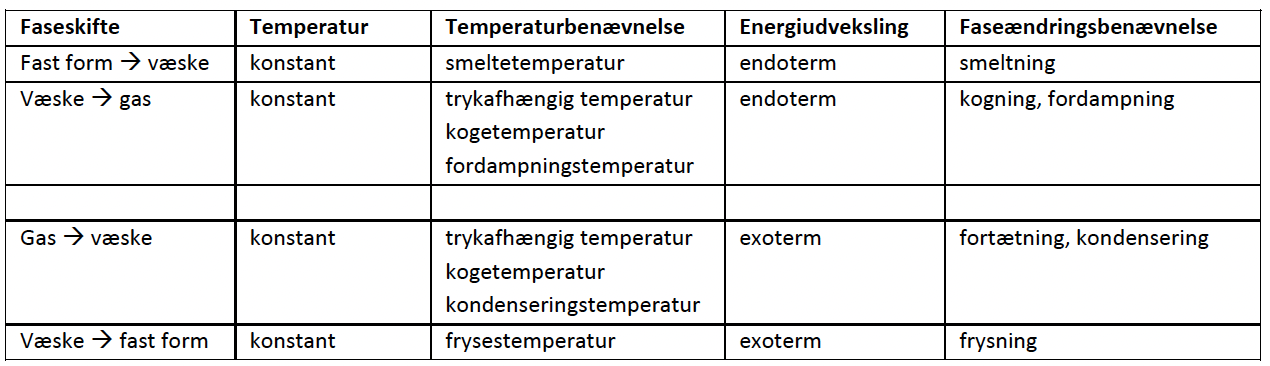
\includegraphics[width=0.5\linewidth]{./figures/f3_2.png}
  \label{fig:f3_2}
\end{figure}

For en kredsproces, hvor der sker faseskift fra f.eks. væske- til gasform og tilbage igen fra gas- til væskeform, vil dette ske ved \textit{konstant} temperatur, såfremt trykket forbliver konstant under hele kredsprocessen (isobarisk proces). At temperaturen forbliver konstant under et faseskift bevirker også at temperaturen ikke kan benyttes som et mål for hvor meget energi, der er optaget. For at imødekomme dette indføres begrebet \textit{gasandel}.

\begin{definition}[Gasandel]
  \textit{Gasandelen}, $x$, defineres som den masse stof, der befinder sig på gasform for en betragtet stofmængde på \qty{1}{kg}. Gasandelen er således en specifik størrelse, der ligger i intervallet $0\leq x\leq 1$. 
\end{definition}

\begin{definition}[Mættet væske]
  En væske, der er tilført en energimængde således, at den ved yderligere tilførsel af energi vil begynde at danne gas, benævnes en \textit{mættet væske}. Her er $x = 0$. 

  Ligeledes har vi, at en stofmængde, som er tilført en energimængde således, at den netop er gå gasform og ved afgivelse af energi vil begynde at danne væskedråber, benævnes en \textit{mættet gas}. Her er $x = 1$. 
\end{definition}

\begin{definition}[Fordampningsvarmen]
  Den energimængde, som skal benyttes for at fordampe et kilogram stofmængde, dvs. skifte fase fra mættet væske til mættet gas kaldes \textit{fordampningsvarmen} og betegnes med symbolet $r_f$. Denne kan findes som $h_{\text{mættet gas}} - h_{\text{mættet væske}}$. 

  Noget tilsvarende gælder for smeltning, hvilket benævnes \textit{smeltningsvarmen} og betenes med symbolet $r_s$. 
\end{definition}

Så længe trykket er konstant har vi at
\[ 
Q_{\text{fordampning}} = Q_{\text{kondensering}} = m \cdot r_f \quad \text{og} \quad Q_{\text{smeltning}} = Q_{\text{frysning}} = m \cdot r_s
.\]

\subsection{Tilstandsdiagrammer}
Et tilstandsdiagram er et koordinatsystem, hvor der på hver akse er en tilstandsstørrelse -- således kan der produceres mange forskellige tilstandsdiagrammer omend kun en håndfuld af disse har reel anvendelse. De mest almindelige tilstandsdiagrammer er:
\begin{itemize}
  \item $p$-$h$ diagram (tryk-entalpi)
  \item $T$-$s$ diagram (temperatur-entropi)
  \item $p$-$v$ diagram (tryk-volumen)
  \item $h$-$s$ diagram (entalpi-entropi)
\end{itemize}

\section{Specifik varmekapacitet og energiberegninger}
\begin{definition}[Specifik varmekapacitet]
  \textit{Den specifikke varmekapacitet} defineres som den varmemængde, der skal bruges for at opvarme \qty{1}{kg} af et givet stof \qty{1}{K}. Denne har symbolet $c$ og enheden $[\unit{\frac{kJ}{\kg.\K}}]$ eller $[\unit{\frac{kJ}{\kg.\celsius}}]$
\end{definition}

For \textit{faste stoffer} er den specifikke varmekapacitet ikke nævneværdigt trykafhængig -- Her er den nærmest udelukkende temperaturafhængig. For \textit{væsker} er den specifikke varmekapacitet i mindre grad afhængig af både tryk og temperatur. For \textit{gasser} er den specifikke varmekapacitet i højere grad afhængig af både tryk og temperatur. Dette medfører også at den specifikke varmekapacitet for en gas ikke er den samme hvis der bliver udført en isokor process på gassen som hvis man udførte en isobar proces på selvsamme gas. Derfor indføres den specifikke varmekapacitet ved konstant volumen $c_v$ og den specifikke varmekapacitet ved konstant tryk $c_p$ defineret som
\begin{align*}
  c_v &= \left( \frac{\partial u}{\partial T} \right)_v \\
  c_p &= \left( \frac{\partial h}{\partial T} \right)_p
.\end{align*}
Idet væsker og faste stoffer er inkompressible vil disse i praksis opleve meget lille forskel mellem $c_v$ og $c_p$ og i stedet benyttes derfor ofte blot en generel varmekapacitet $c$. 

Med afsæt i ovenstående kan den absolutte energimængde $Q$ for hhv. et isobarisk og isokorisk procesforløb bestemmes som
\begin{align*}
  Q_{\text{isok}} &= m\cdot c_{v, m} \cdot \left( T_2 - T_1 \right) \\
  Q_{\text{isob}} &= m \cdot c_{p, m}\cdot \left( T_2 - T_1 \right)
.\end{align*}

Faktisk kan det også vises at differensen mellem den specifikke varmekapacitet ved konstant tryk $c_p$ og den specifikke varmekapacitet ved konstant volumen $c_v$ (for en idealgas) netop er den individuelle gaskonstant $R_i$ som
\[ 
c_p - c_v = R_i
.\]

Forholdet mellem den specifikke varmekapacitet ved hhv. konstant tryk of volumen benævnes \textit{isentropeksponenten} $\kappa$:
\[ 
\kappa = \frac{c_p}{c_v} = 1 + \frac{R_i}{c_v}
.\]
